\section{Results}
\subsection{Parameter Descriptions}
\begin{table}
\centering
\caption{Hyperparameter Legend}
\label{tab:hyplegend}
\begin{tabular}{lll}
\toprule
{} & Hyperparameter &                                       Description \\
\midrule
0 &     layer\_type &      the type of DNN layer used in the experiment \\
1 &   layer2\_units &           number of nodes in the 1st hidden layer \\
2 &   layer3\_units &           number of nodes in the 2nd hidden layer \\
3 &     activation &  activation function used for layers in the model \\
4 &      optimizer &                     optimizer used while training \\
5 &           loss &                  the loss metric used in training \\
6 &        dropout &                      the dropout used in training \\
\bottomrule
\end{tabular}
\end{table}
\subsection{Summary of Analysis}
\begin{table}
\centering
\caption{Top 5 Model Confusion Matrices Selected by Highest Average f1 Score Across Thresholds [0.3, 0.5, 0.7]}
\label{tab:summary_confmatrix}
\begin{tabular}{lrrrr}
\toprule
{} &  accuracy &  precision &    recall &  f1 score \\
model\_no                     &           &            &           &           \\
\midrule
Model\_Weight\_\#20210319135523 &  0.840671 &   0.862617 &  0.830383 &  0.841772 \\
Model\_Weight\_\#20210319135331 &  0.836859 &   0.862522 &  0.821165 &  0.837258 \\
Model\_Weight\_\#20210319135536 &  0.834953 &   0.861593 &  0.820059 &  0.834907 \\
Model\_Weight\_\#20210319135849 &  0.833047 &   0.856172 &  0.823009 &  0.834309 \\
Model\_Weight\_\#20210319135101 &  0.834572 &   0.863253 &  0.818584 &  0.834038 \\
\bottomrule
\end{tabular}
\end{table}
\subsection{Experiment 20210319134850\_seed1}
\subsubsection{Model Model\_Weight\_\#20210319135523}

        \begin{figure}
        \caption{Network model for 20210319134850\_seed1 Model\_Weight\_\#20210319135523}
        \centering
            \includegraphics[width=0.5\linewidth]{20210319134850_seed1/ModelWeight20210319135523/model_struct.png}
        \label{fig:20210319134850seed1/ModelWeight20210319135523/modelstruct.png}
        \end{figure}
        \begin{table}
\centering
\caption{Confusion Matrix for 20210319134850\_seed1 Model\_Weight\_\#20210319135523}
\label{tab:conf_matr20210319134850seed1ModelWeight20210319135523}
\begin{tabular}{lrrrr}
\toprule
{} &  accuracy &  precision &    recall &  f1 score \\
threshold &           &            &           &           \\
\midrule
0.3       &  0.851344 &   0.818182 &  0.915929 &  0.864301 \\
0.5       &  0.848485 &   0.853821 &  0.852876 &  0.853348 \\
0.7       &  0.822184 &   0.915849 &  0.722345 &  0.807669 \\
\bottomrule
\end{tabular}
\end{table}
\begin{table}
\centering
\caption{Hyperparameter's for 20210319134850\_seed1 Model\_Weight\_\#20210319135523}
\label{tab:hyp20210319134850seed1ModelWeight20210319135523}
\begin{tabular}{lll}
\toprule
{} & Hyperparameter &                Value \\
\midrule
0 &     layer\_type &                dense \\
1 &   layer2\_units &                   36 \\
2 &   layer3\_units &                   12 \\
3 &     activation &                lrelu \\
4 &      optimizer &                 Adam \\
5 &           loss &  binary\_crossentropy \\
6 &        dropout &                  0.1 \\
7 &          alpha &                  0.3 \\
8 &     num\_epochs &                   50 \\
9 &     batch\_size &                   50 \\
\bottomrule
\end{tabular}
\end{table}
\subsubsection{Model Model\_Weight\_\#20210319135331}

        \begin{figure}
        \caption{Network model for 20210319134850\_seed1 Model\_Weight\_\#20210319135331}
        \centering
            \includegraphics[width=0.5\linewidth]{20210319134850_seed1/ModelWeight20210319135331/model_struct.png}
        \label{fig:20210319134850seed1/ModelWeight20210319135331/modelstruct.png}
        \end{figure}
        \begin{table}
\centering
\caption{Confusion Matrix for 20210319134850\_seed1 Model\_Weight\_\#20210319135331}
\label{tab:conf_matr20210319134850seed1ModelWeight20210319135331}
\begin{tabular}{lrrrr}
\toprule
{} &  accuracy &  precision &    recall &  f1 score \\
threshold &           &            &           &           \\
\midrule
0.3       &  0.849628 &   0.820180 &  0.908186 &  0.861942 \\
0.5       &  0.839909 &   0.852941 &  0.834071 &  0.843400 \\
0.7       &  0.821041 &   0.914446 &  0.721239 &  0.806432 \\
\bottomrule
\end{tabular}
\end{table}
\begin{table}
\centering
\caption{Hyperparameter's for 20210319134850\_seed1 Model\_Weight\_\#20210319135331}
\label{tab:hyp20210319134850seed1ModelWeight20210319135331}
\begin{tabular}{lll}
\toprule
{} & Hyperparameter &                Value \\
\midrule
0 &     layer\_type &                dense \\
1 &   layer2\_units &                   36 \\
2 &   layer3\_units &                   12 \\
3 &     activation &                lrelu \\
4 &      optimizer &                 Adam \\
5 &           loss &  binary\_crossentropy \\
6 &        dropout &                  0.1 \\
7 &          alpha &                  0.3 \\
8 &     num\_epochs &                   50 \\
9 &     batch\_size &                    5 \\
\bottomrule
\end{tabular}
\end{table}
\subsubsection{Model Model\_Weight\_\#20210319135536}

        \begin{figure}
        \caption{Network model for 20210319134850\_seed1 Model\_Weight\_\#20210319135536}
        \centering
            \includegraphics[width=0.5\linewidth]{20210319134850_seed1/ModelWeight20210319135536/model_struct.png}
        \label{fig:20210319134850seed1/ModelWeight20210319135536/modelstruct.png}
        \end{figure}
        \begin{table}
\centering
\caption{Confusion Matrix for 20210319134850\_seed1 Model\_Weight\_\#20210319135536}
\label{tab:conf_matr20210319134850seed1ModelWeight20210319135536}
\begin{tabular}{lrrrr}
\toprule
{} &  accuracy &  precision &    recall &  f1 score \\
threshold &           &            &           &           \\
\midrule
0.3       &  0.846770 &   0.813609 &  0.912611 &  0.860271 \\
0.5       &  0.844483 &   0.851111 &  0.847345 &  0.849224 \\
0.7       &  0.813608 &   0.920058 &  0.700221 &  0.795226 \\
\bottomrule
\end{tabular}
\end{table}
\begin{table}
\centering
\caption{Hyperparameter's for 20210319134850\_seed1 Model\_Weight\_\#20210319135536}
\label{tab:hyp20210319134850seed1ModelWeight20210319135536}
\begin{tabular}{lll}
\toprule
{} & Hyperparameter &                Value \\
\midrule
0 &     layer\_type &                dense \\
1 &   layer2\_units &                   36 \\
2 &   layer3\_units &                   12 \\
3 &     activation &                lrelu \\
4 &      optimizer &                 Adam \\
5 &           loss &  binary\_crossentropy \\
6 &        dropout &                  0.2 \\
7 &          alpha &                  0.3 \\
8 &     num\_epochs &                   50 \\
9 &     batch\_size &                   50 \\
\bottomrule
\end{tabular}
\end{table}
\subsubsection{Model Model\_Weight\_\#20210319135849}

        \begin{figure}
        \caption{Network model for 20210319134850\_seed1 Model\_Weight\_\#20210319135849}
        \centering
            \includegraphics[width=0.5\linewidth]{20210319134850_seed1/ModelWeight20210319135849/model_struct.png}
        \label{fig:20210319134850seed1/ModelWeight20210319135849/modelstruct.png}
        \end{figure}
        \begin{table}
\centering
\caption{Confusion Matrix for 20210319134850\_seed1 Model\_Weight\_\#20210319135849}
\label{tab:conf_matr20210319134850seed1ModelWeight20210319135849}
\begin{tabular}{lrrrr}
\toprule
{} &  accuracy &  precision &    recall &  f1 score \\
threshold &           &            &           &           \\
\midrule
0.3       &  0.838765 &   0.801357 &  0.914823 &  0.854339 \\
0.5       &  0.843339 &   0.854730 &  0.839602 &  0.847098 \\
0.7       &  0.817038 &   0.912429 &  0.714602 &  0.801489 \\
\bottomrule
\end{tabular}
\end{table}
\begin{table}
\centering
\caption{Hyperparameter's for 20210319134850\_seed1 Model\_Weight\_\#20210319135849}
\label{tab:hyp20210319134850seed1ModelWeight20210319135849}
\begin{tabular}{lll}
\toprule
{} & Hyperparameter &                Value \\
\midrule
0 &     layer\_type &                dense \\
1 &   layer2\_units &                   36 \\
2 &   layer3\_units &                   12 \\
3 &     activation &                lrelu \\
4 &      optimizer &                 Adam \\
5 &           loss &  binary\_crossentropy \\
6 &        dropout &                  0.1 \\
7 &          alpha &                  0.5 \\
8 &     num\_epochs &                   50 \\
9 &     batch\_size &                   50 \\
\bottomrule
\end{tabular}
\end{table}
\subsubsection{Model Model\_Weight\_\#20210319135101}

        \begin{figure}
        \caption{Network model for 20210319134850\_seed1 Model\_Weight\_\#20210319135101}
        \centering
            \includegraphics[width=0.5\linewidth]{20210319134850_seed1/ModelWeight20210319135101/model_struct.png}
        \label{fig:20210319134850seed1/ModelWeight20210319135101/modelstruct.png}
        \end{figure}
        \begin{table}
\centering
\caption{Confusion Matrix for 20210319134850\_seed1 Model\_Weight\_\#20210319135101}
\label{tab:conf_matr20210319134850seed1ModelWeight20210319135101}
\begin{tabular}{lrrrr}
\toprule
{} &  accuracy &  precision &    recall &  f1 score \\
threshold &           &            &           &           \\
\midrule
0.3       &  0.845626 &   0.812008 &  0.912611 &  0.859375 \\
0.5       &  0.846198 &   0.849285 &  0.853982 &  0.851627 \\
0.7       &  0.811893 &   0.928465 &  0.689159 &  0.791111 \\
\bottomrule
\end{tabular}
\end{table}
\begin{table}
\centering
\caption{Hyperparameter's for 20210319134850\_seed1 Model\_Weight\_\#20210319135101}
\label{tab:hyp20210319134850seed1ModelWeight20210319135101}
\begin{tabular}{lll}
\toprule
{} & Hyperparameter &                Value \\
\midrule
0 &     layer\_type &                dense \\
1 &   layer2\_units &                   36 \\
2 &   layer3\_units &                   12 \\
3 &     activation &                lrelu \\
4 &      optimizer &                 Adam \\
5 &           loss &  binary\_crossentropy \\
6 &        dropout &                  0.2 \\
7 &          alpha &                  0.1 \\
8 &     num\_epochs &                   50 \\
9 &     batch\_size &                    5 \\
\bottomrule
\end{tabular}
\end{table}
